\documentclass[12pt]{article}

\usepackage{amsmath, amsthm, amssymb, amsfonts, appendix}
\usepackage{graphicx, float}


\def\RR{{\mathbb R}}
\def\CC{{\mathbb C}}

\title{%
	Visualizing Julia Sets \\
	\large An Algorithmic Approach
	
	}
\author{Wyatt Whiting}

\begin{document}
\maketitle

\begin{abstract}
In this paper, we present a definition of the Julia set for a  complex-valued function $f:Z\rightarrow Z$. The conditions for $f$ necessary to define an associated Julia set are presented and discussed. Finally, we discuss an algorithmic method for producing visualizations of Julia sets.
\end{abstract}

\section{Introduction}

Before we can discuss the properties of Julia sets, we must begin with a formal definition of precisely what they are. We first note that there is no \textit{one} Julia set. Rather, Julia sets correspond to functions such that, given two functions $f$ and $g$ such that $f \not\equiv g$, then the corresponding Julia sets are possibly unique (more on this later). While one could consider the set of only real-valued functions, the far more interesting results come from the consideration of complex-valued functions.

\subsection{Complex Prerequisites}

As we are discussing complex functions, it is therefore necessary to have some understanding of the terminology relating to these functions. We'll start by defining the imaginary unit $i$:

\subsubsection{Imaginary Unit and Complex Numbers}

\theoremstyle{definition}%
\newtheorem{defin}{Defintion}
\begin{defin} The imaginary unit $i$ is a number such that
\[
i^2 = -1.
\]
\end{defin}

Complex numbers have a real and imaginary component:

\begin{defin} A complex number $z$ is a number such that
\[
z=a+bi, \quad a,b\in\RR.
\]
\end{defin}

Just as for any real number $x$, we an say that $x\in\RR$, we say that for any complex number $z$, we have $z\in\CC$ where $\CC$ denotes the set of complex numbers. 

There is a natural method of plotting complex numbers. Given some $z=a+bi$, we can plot the point $(a,b)$ in $\RR^2$ to represent the point. As complex numbers are comprised of two real coefficients, then we can associate every unique complex number with a single point. In this way, we avoid any "collisions" in plotting the complex numbers. 

\subsubsection{Complex Polynomials}

Complex numbers likewise have a number of operations on them we will need. One may add two complex numbers together to get another complex number, and multiply them together as well. With these two operations, we can construct complex polynomials. 

\begin{defin} A complex polynomial is a polynomial equation with complex-valued coefficients.
\end{defin}

Finally, we must consider the concept of complex differentiability. Just as one can differentiate real-valued functions, one may differentiate complex-valued functions as well. The complex derivative by the limit

\begin{equation}
f'(z_0) = \lim_{z\to z_0} \frac{f(z)-f(z_0)}{z-z_0}.
\end{equation} 
 
One might notice that this definition is identical to the limit definition of the derivative on real values, given by 

\begin{equation}
f'(x_0) = \lim_{x\to x_0}\frac{f(x)-f(x_0)}{x-x_0}.
\end{equation}
 
It is no coincidence that these definitions are analogous. In fact, virtually all things we may do with real-valued functions, we may do with complex-valued functions as well.

\subsubsection{Holomorphism}

Finally, we are able to define the last bit of machinery we will need for discussion of Julia sets. This is the idea of a "holomorphic function."

\begin{defin}
A complex-valued function $f:\CC\to\CC$ is called holomorphic if, at every point in it's domain, it is complex differentiable in a neighborhood around that point, as well as being locally equal to its own Taylor series. 
\end{defin}
 
The concept of Taylor series is analogous between real- and complex-valued functions. The only difference being that the Taylor series of a complex-valued function may have complex-valued coefficients. As the Taylor series itself creates a polynomial, it should make sense that one may create a Taylor polynomial which is exactly equal to the complex polynomial itself. We may then assert that all complex polynomials are holomorphic. 
% NOTE: Maybe find reference for this somewhere? check old complex analysis textbook



\subsection{Defining Julia Sets}

As Julia sets are associated with functions, we first define the types of functions we care about. Let $f :\CC\to\CC$ be a complex-valued, non-constant holomorphic function. For the purposes of this paper, we will take 

\begin{equation}
f_C(z) = z^2 + C, \quad C \in \CC.
\end{equation}

to be our function. However, we can choose $f_C$ to be \textit{any} function which satisfies the necessary conditions. In its most general form, $f_C$ can be any nonconstant complex rational functions of the form $f_C(z) = p(z)/q(z)$, where $p$ and $q$ are complex polynomials which share no common roots and at least one has degree of at least $1$. We can see that $f_C(z) = z^2 + C$ satisfies this condition, as we can take

\begin{align*}
p(z) &= z^2 + C, \\
q(z) &= 1, \\
\implies p(z)/q(z) &= \frac{z^2 + C}{1} = z^2 + C, \\
&= f_C(z).
\end{align*}

We now may make a statement about exactly \textit{what} a Julia set is. 

\begin{defin}
A Julia set of a function, denoted $J(f)$, is the boundary of the set of points in the complex plane which converge to infinity under iteration of $f$ \cite{Milnor}. 
\end{defin}

This is a somewhat unwieldy definition, so let's attempt to make this a bit more clear. 

Take a point on the complex plane. WLOG, we can just call this point $z_0 = a_0 + b_0i$, which has some magnitude $|z_0| = |a_0 + b_0i| = \sqrt{a_0^2 + b_0^2}$. If we pass this complex number into $f_C$, we get a (possibly) new complex number, $f(z_0) = z_0^2 + C = z_1 = a_1 + b_1i$ with magnitude $|z_1| = \sqrt{a_1^2 + b_1^2}$. By continuing this process, we generate a chain of complex numbers $\{ z_0, z_1, z_2, z_3, \cdots \}$. This chain can either stay bounded to a region of the complex plane near the origin under repeated iteration, or it can "explode" away from the origin such that, if we let the function iterate an infinite number of times, $|z_i|\to\infty$. 

We can then think about two "types" of points: those that stay bounded under repeated iteration of $f_C$, and those who do not stay bounded. $J(f)$ is then the points that are on the boundary of those which stay bounded, and those which "blow up" to have infinite magnitude. We note there is a "critical radius" $R > 0$ such that, given some $z\in\CC$ where $|z| > R^2$, then we know that $z$ will only increase in magnitude after applying $f_C$. If we choose $R$ such that

\begin{align*}
R^2 - R &\geq |z| \\
\implies R &= \frac{1}{2}\left(1+\sqrt{1 + 4|z|} \right),
\end{align*}

then we know that if $|z| > R \implies |f_C(z)| > |z| > R$, so the magnitude will only increase with further iterations. 

\section{Visualization Method}

Now equipped with some understanding of exactly what $J(f)$ \textit{is}, we can go about calculating and and visualizing what these sets look like. To this end, we will describe an algorithm which creates a visual approximation of $J(f)$ for some given constant $C$. We say this visualization is only an approximation because we are not able to iterate over every point an infinite number of times, and because we can only carry out the determination algorithm for a finite set of points. If we were to calculate the \textit{true} set, we would have to calculate an uncountably infinite number of points with a countably infinite of iterations on each point to determine whether that point stays bounded under iteration or whether is blows off to infinity. By taking advantage of the critical radius, we know that points which end up outside the radius will blow up to infinity

\subsection{Algorithm presented}

The first thing we must do is create an $n \times m$ matrix of complex values that are evenly spaced inside some bounding box we specify. For a very simple example, let's look at what this matrix would look like for a $3 \times 3$ matrix inside the bounding box $[-1, 1] \times i[-1, 1]$:

\begin{equation*}
\begin{bmatrix}
-1 + i & 0 + i & 1 + i \\
-1 & 0 & 1 \\
-1-i & 0-i & 1-i
\end{bmatrix}
\end{equation*}

We then apply the following algorithm to each entry of the matrix to determine the "escape number" for each starting value:

\begin{enumerate}
	\item Select a starting point, $z$. 
	\item Update your pointer by iteration with $f_C$ to $z_0$, such that $z = f_C(z)$.
	\item Increment counter which tracks number of iterations applied. 
	\item Check whether point is outside of a critical radius R.
	\begin{itemize}
		\item If so, terminate function and return the iteration count
	\end{itemize}
	\item Check if number of iterations exceed maximum number of iterations allowed
	\begin{itemize}
		\item If so, terminate function and return iteration count
	\end{itemize}
	\item Return to step $2.$
	
\end{enumerate}

We simply apply this algorithm to the set of points we want to check, and then translate the number of 

We set a maximum number of iterations to avoid infinite loops. If a starting point of the algorithm truly does stay bounded regardless of how many iterations we allowed, we would be stuck in an infinite loop, which is clearly undesirable behavior. However, this does lead to some degree of inaccuracy in the method. This is because only know that the point stays bounded \textit{within that number of iterations}. It is entirely possible that, given more iterations, that point will eventually escape the critical radius. This is simply just a reality we have to accept, and by choosing a sufficiently large maximum iteration number, we can produce a visual result that is "close enough" to the true set. 

\subsection{Implementation}

The implementation of this in MATLAB can be found in Appendix A. 

\section{Results}

\subsection{Standard Function}

We now present the results of running the plotting function with the "standard" function, $f(z) = z^2 + C$. Each image will be presented with the complex parameter $C$ which leads to that particular plot. All plots, unless noted otherwise, will be plotted for complex numbers $z\in \{[-1.7, 1.7]\times i[-1.7, 1.7]\}$.

\subsubsection{$f_C = z^2 + C$}

First, let's look at what happens when $C = 0$.

\begin{figure}[H]
	\centering
	
\includegraphics[scale=0.5]{Ceq0.png}
	\caption{Julia set for $f_C = z^2 + 0$}
\end{figure}

As we can see, this is just a circle. We find this to be the case because complex numbers with a magnitude less or equal to 1 will stay within the unit circle under squaring, and those outside will have their magnitude only increase. Therefore, we end up seeing a circle. 

\subsubsection{$f_C = z^2 + i$}

For each iteration, let's add the imaginary unit after squaring the complex number: 

\begin{figure}[H]
	\centering
	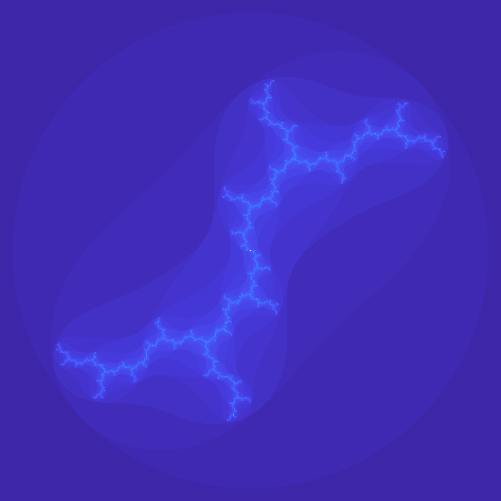
\includegraphics[scale=0.5]{Ceqi.png}
	\caption{Julia set for $f_C = z^2 + i$}
\end{figure}

We can see we don't get a nicely yellow region, which would indicate that points in that region all stay bounded. Rather, we end up with a strange, lightning-like tendrils. We also note that the figure has rotational symmetry around the origin. In this case, it seems to be the case that all points end up escaping to infinity. However, not all points do this at the same rate. Some take only a few iterations, while others "linger" for a while. The coloring scheme from MATLAB assigns different colors to the number of iterations, allowing us to see this variation. 

\subsubsection{$f_C = z^2 - 0.4 + 0.6i$} 

\begin{figure}[H]
	\centering
	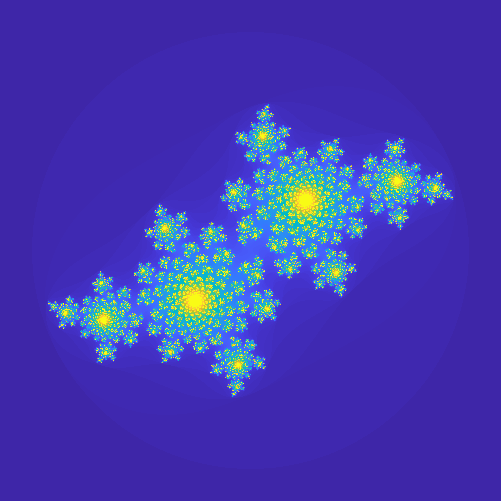
\includegraphics[scale=0.5]{Ceqm0406.png}
	\caption{Julia set for $f_C = z^2 - 0.4 + 0.6i$}
\end{figure}

With this value for $C$, we get a highly intricate pattern. It is now clear to see the fractal structure of the plot: if one examines closely, you can see how separate clusters of color are identical to other clusters, the only difference being a pan, rotate, and scale. We also note that the figure maintains rotational symmetry (in fact, all plots coming from the function in the form $z^2 + C$ will have rotational symmetry in this way). 

We could generate an infinite number of plots, each unique from the last, but for the sake of brevity, we will stop the exploration of these "standard" plots. 

\subsection{Departing from the Standard}

We previously were exploring plots coming from the function $f_C(z) = z^2 + C$. However, the definition of $J(f)$ does not necessitate this. Let's play around with the function we are using and see what we can come up with.

\subsubsection{$f_C = z^n + C$}

If functions that square $z$ have two sides, what about functions that cube $z$?

\begin{figure}[H]
	\centering
	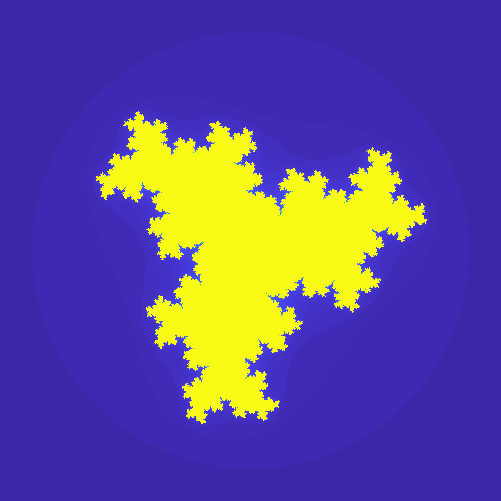
\includegraphics[scale=0.5]{cube.png}
	\caption{Julia set for $f_C = z^3 - 0.4 + 0.6i$}
\end{figure}

We get three lobes! What if we try, say, raising $z$ to the 7th power?

\begin{figure}[H]
	\centering
	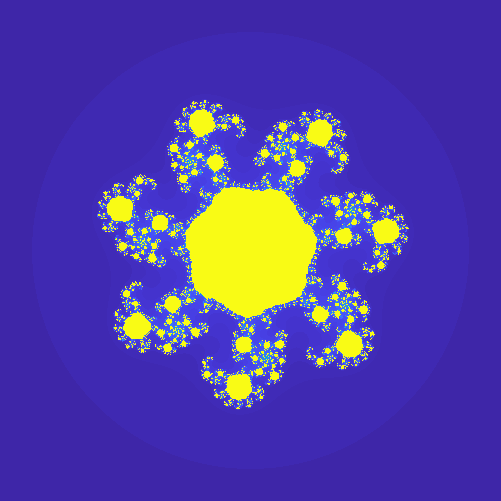
\includegraphics[scale=0.5]{seven.png}
	\caption{Julia set for $f_C = z^7 - 0.4 + 0.6i$}
\end{figure}

We end up with 7 lobes, and we maintain rotational symmetry. Let's try something more exotic next.

\subsubsection{Irrational and Complex Powers}

What happens if we raise $z$ to an irrational power, say $\sqrt{3}$?

\begin{figure}[H]
	\centering
	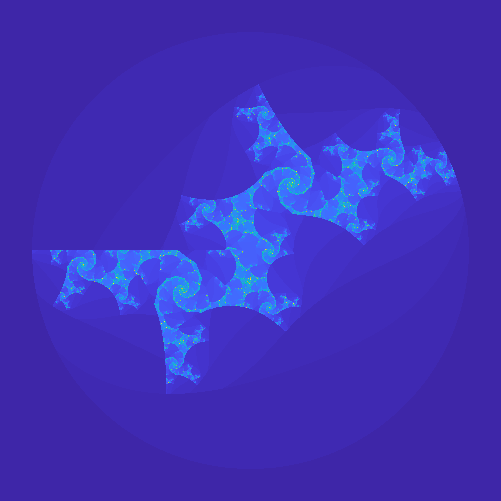
\includegraphics[scale=0.5]{root3_0.png}
	\caption{Julia set for $f_C = z^{\sqrt{3}} - 0.4 + 0.6i$}
\end{figure}

Here we get a beautiful ghost-like pattern, which has \textit{nearly} rotational symmetry. We can observe two large swirls near the center which appear to be the same, but the figure as a whole does not have rotational symmetry. Since $sqrt{3}\approx 1.73..$ is close to 2, then the resulting figure has \textit{nearly} two-way symmetry. 

Let's try raising $z$ to a complex power:

\begin{figure}[H]
	\centering
	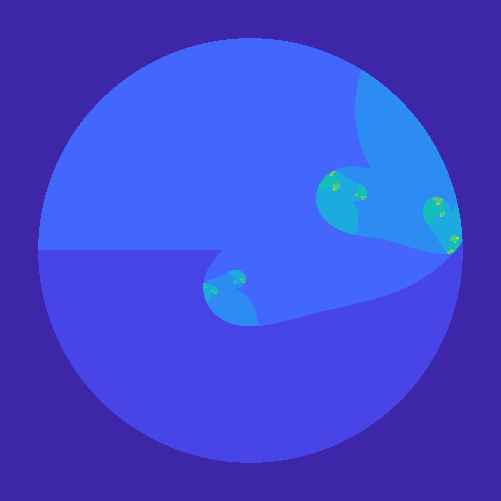
\includegraphics[scale=0.5]{complexPow.png}
	\caption{Julia set for $f_C = z^{2 - i} - 0.4 + 0.5i$}
\end{figure}

Here we get a strange set of dust-like points which linger, and possibly only a few, disconnected points which stay bounded. If we were able to interactively zoom into those parts of the figure, perhaps we would discover some interesting structure which is too fine to perceive here. 

\section{Conclusion}

As we can see, there are an infinite number of Julia sets coming from an infinite number of functions. When visualized, these graphs can result in a huge variety of possible figures, ranging wildly in structure and symmetry. While being interesting for those familiar with the mathematics behind the generation of the figures, these can be artistically intriguing to non-mathematical laypeople as well. 

Without rigorous proof, we present a number of observations we expect to hold. For graphs generated by functions of the form $f_C = z^n + C$ where $n\geq 2$, the resulting figure will have $n$ ways of rotational symmetry. Furthermore, when $n$ is an irrational number greater than $1$, the resulting figure will have no rotational symmetry. Finally, we notice that some figures have nice, solid regions of continuity, and others have frenetic and disconnected regions where no continuous regions collectively stay bounded under iteration. 

In fact, given the constant from that function $C$, the resulting figure will have a solid, well-defined region if and only if $C$ is included in the Mandlebrot Set for that particular function \cite{Lei89}. 

I highly encourage the reader to take the code found in Appedix A and generate your own figures. While we have presented a number of interesting ones here, there were dozens more that we were not able to fit into this paper.





\appendix
\section{MATLAB code}
The MATLAB code consists of two \texttt{.m} files: one for underlying code to generate and return an array of iteration counts from a vector of input parameters, and a second to drive the code. The underlying logic is implemented in \texttt{param\_to\_image.m}, and the driver is implemented in \texttt{static\_image.m}. 

\bigskip

\texttt{static\_image.m}:
\begin{verbatim}
% parameters for image
% bounds for plotting
RE_MIN = -1.7;
RE_MAX =  1.7;
IM_MIN = -1.7;
IM_MAX =  1.7;
% real and imaginary resolution
RE_RES = 5001;
IM_RES = 5001;
% complex constant C
C = complex(-0.2, -sqrt(2)/2);
% maximum number of iterations for algorithm to run
MAX_ITER = 80;
% power for Z
POW = 2;

% create vector of values to easy passing
vec = [RE_MIN RE_MAX RE_RES IM_MIN IM_MAX IM_RES C MAX_ITER POW];

% below is the non-saving version for exploring images.
% It displays the image created by all the given parameters
imagesc(param_to_image(vec));
% uncomment line below to save image automatically
% WARNING: requires image processing toolkit.
% imwrite( ind2rgb(im2uint8(mat2gray(param_to_image(vec))), ...
  parula(256)), './test.png');
\end{verbatim}

\bigskip

And now \texttt{param\_to\_image.m}:
\begin{verbatim}
function out = param_to_image(vec)
    % output the count_grid function
    % applied to every element from the 
    % result of complex_grid, which
    % each take arguments from the 'global'
    % argument vector 'vec'.
    out = arrayfun(@(z) count_grid(z, vec), complex_grid(vec));
end

% count_grid takes in a complex starting point and 
% returns an interation count
function out = count_grid(A, in)
    % set escape radius
    R = (1/2) * (1 + sqrt(1 + 4*abs(in(7))));
    
    % initialize iteration count
    iter = 0;
    
    % loop while magnitude is within critical radius and
    % maximum iteration count has not been met
    while abs(A) < R && iter < abs(in(8))
        % apply iteration and increment count
        A = A^(in(9)) + in(7);
        iter = iter + 1;
    end
    % after loop terminates, return the number of iterations
    out = iter;
end

% complex_grid returns a matrix of complex values
% with bounds specified by the argument vector 'in'
function out = complex_grid(in)
    % linear space of strictly real values
    x = complex(linspace(in(1), in(2), in(3)));
    % linear space of strictly imaginary values
    y = complex(0,linspace(in(4), in(5), in(6)));
    % create mesgrid of both linear spaces
    [x, y] = meshgrid(x, y);
    % sum ends up being the spaving we want for evenly
    % placed points in the complex plane
    out = x + y;
end
\end{verbatim}

\begin{thebibliography}{1}

\bibitem{Lei89} Tan Lei {\em Similarity between the Mandelbrot Set and Julia Sets}, Communications in Mathematical Physics, 10 July 1989.

\bibitem{Milnor} John Milnor {\em DYNAMICS IN ONE COMPLEX VARIABLE}, Institute for Mathematical Sciences,  SUNY, 5 September 1991. 

\end{thebibliography}

\end{document}

